%%%%%%%%%%%%%%%%%%%%%%%%%%%%%%%%%%%%%%%%%%%%%%%%%%%%%%%%%%%%%%%%%%
%%%
%%%                   report_template_LaTeX
%%%                          main.tex
%%%   <https://github.com/matsukawa-group/report_template_LaTeX>
%%%
%%%%%%%%%%%%%%%%%%%%%%%%%%%%%%%%%%%%%%%%%%%%%%%%%%%%%%%%%%%%%%%%%%

%%% 文書クラスの設定 %%%
\documentclass[
    paper=a4paper,      % A4 用紙サイズ
    article,            % article 相当の文書クラス
    fontsize=11pt,      % 欧文サイズ 11 pt
    jafontsize=11pt,    % 和文サイズ 11 pt
    head_space=25mm,    % 天の余白
    foot_space=25mm,    % 地の余白
    gutter=20mm,        % のどの余白
    fore-edge=20mm      % 小口の余白
    ]{jlreq}            % jlreq クラスを使用

%==================================================
% パッケージの読み込み
%==================================================

\usepackage{settings}

% 読み込む bib ファイル（複数ある場合は \addbibresource を並べる）
\addbibresource{bibliography.bib}

%==================================================
% 基本設定
%==================================================

% 文書タイトル
\newcommand{\DocTitle}{%
  ここに文書のタイトルを入れます
}

% 日付
\newcommand{\DocDate}{%
  2026 年 6 月 1 日%
}

% 表紙を付けるかどうか
\newif\ifcover
\covertrue
% \coverfalse

%==================================================
% 著者の登録
%==================================================

\addauthor
  {著者名}
  {著者の所属・学年}
  {author@example.com}

% 第二著者を追加する場合
%
% \addauthor
%   {第二著者}
%   {第二著者の所属・学年}
%   {second@example.com}


%==================================================
% 本文
%==================================================

\begin{document}

% \maketitle
\makedocumenttitle

\thispagestyle{cover}

% 目次が不要な場合はコメントアウト
\tableofcontents
\clearpage

\section{これは見出し}
\label{sec:heading}

\subsection{これは小見出し}
\label{ssec:subheading}

\subsubsection{これはさらに小さい見出し}
\label{sssec:subsubheading}

コピペ用に図と表はここにも置いておきます．
その他は \verb|template-manual/| ディレクトリのファイルを参考にしてください．

\clearpage

%%% 図を 1 枚だけ配置するときはこれをコピーアンドペーストすればよい．
\begin{figure}[t]
    \centering
    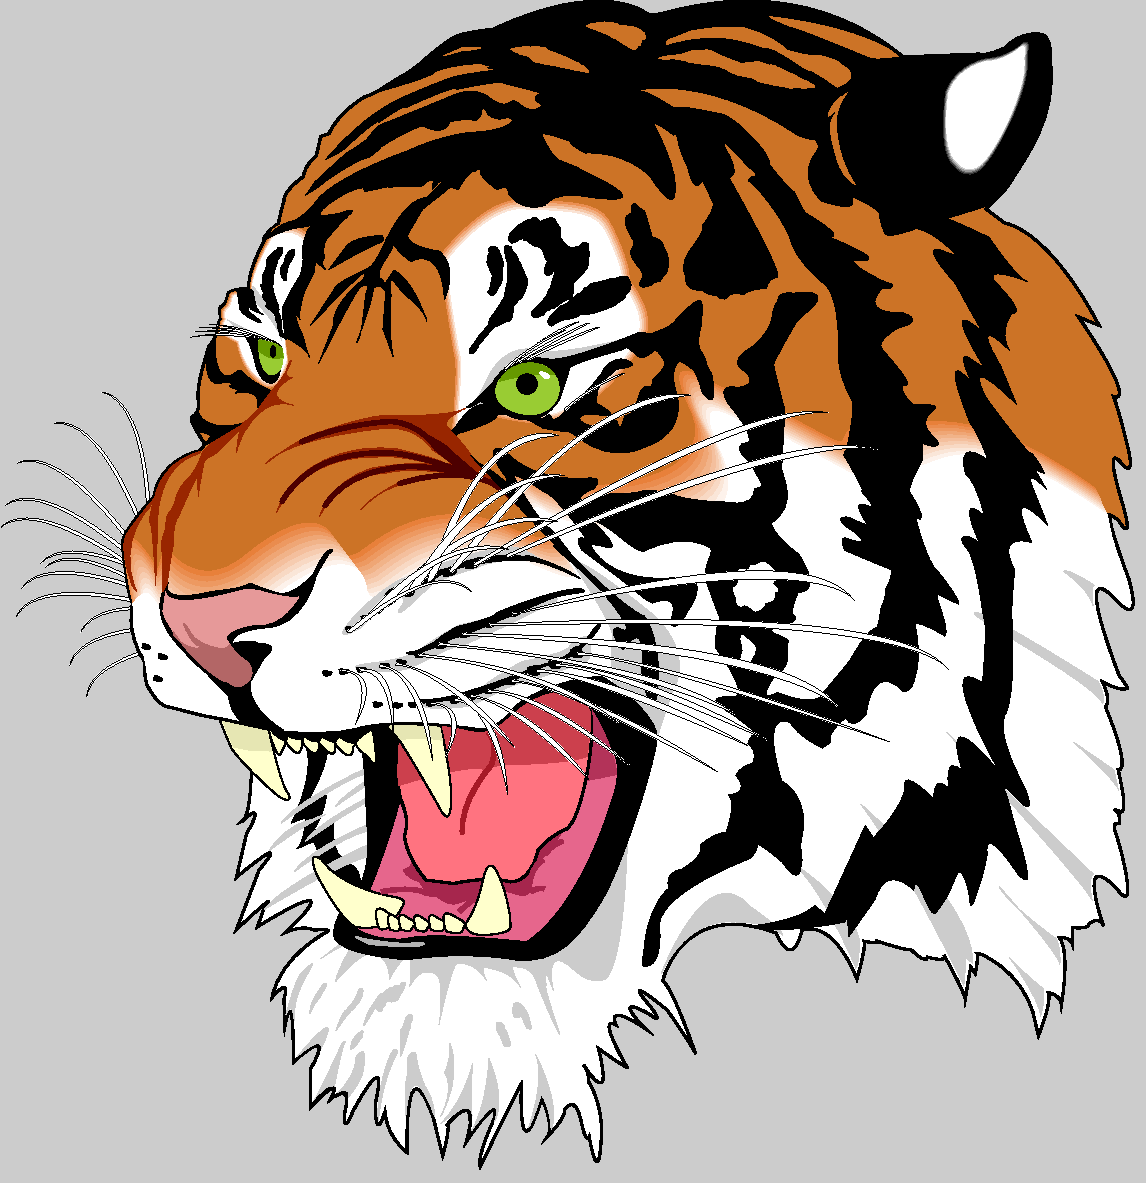
\includegraphics[width=0.6\columnwidth]{figure/tiger.pdf}
    \caption{Please write the figure caption here.}
    \label{fig:one_figure}
\end{figure}
%%%

%%% 図を 2 枚横並びで配置するときはこれをコピーアンドペーストすればよい．
\begin{figure}[t]
    \centering
    \begin{subfigure}{0.45\columnwidth}
        \centering
        \includegraphics[width=\columnwidth]{example-image-a}
        \caption{Left figure caption.}
        \label{subfig:two_figures_a}
    \end{subfigure}
    \hfill % ここで空白を入れると図が適切に配置される
    \begin{subfigure}{0.45\columnwidth}
        \centering
        \includegraphics[width=\columnwidth]{example-image-b}
        \caption{Right figure caption.}
        \label{subfig:two_figures_b}
    \end{subfigure}
    \caption{Two figures placed side by side.}
    \label{fig:two_figures}
\end{figure}
%%%

%%% 図を 3 枚横並びで配置するときはこれをコピーアンドペーストすればよい．
\begin{figure}[t]
    \centering
    \begin{subfigure}{0.32\columnwidth}
        \centering
        \includegraphics[width=\columnwidth]{example-image-a}
        \caption{Left figure caption.}
        \label{subfig:three_figures_a}
    \end{subfigure}
    \hfill % ここで空白を入れると図が適切に配置される
    \begin{subfigure}{0.32\columnwidth}
        \centering
        \includegraphics[width=\columnwidth]{example-image-b}
        \caption{Center figure caption.}
        \label{subfig:three_figures_b}
    \end{subfigure}
    \hfill % ここで空白を入れると図が適切に配置される
    \begin{subfigure}{0.32\columnwidth}
        \centering
        \includegraphics[width=\columnwidth]{example-image-c}
        \caption{Right figure caption.}
        \label{subfig:three_figures_c}
    \end{subfigure}
    \caption{Three figures placed side by side.}
    \label{fig:three_figures}
\end{figure}
%%%

%%% 図を 4 枚上下左右に配置するときはこれをコピーアンドペーストすればよい．
\begin{figure}[t]
    \centering
    % 上の行
    \begin{subfigure}{0.45\columnwidth}
        \centering
        \includegraphics[width=\columnwidth]{example-image-a}
        \caption{Upper-left figure caption.}
        \label{subfig:four_figures_a}
    \end{subfigure}
    \hfill % 水平方向のスペース
    \begin{subfigure}{0.45\columnwidth}
        \centering
        \includegraphics[width=\columnwidth]{example-image-b}
        \caption{Upper-right figure caption.}
        \label{subfig:four_figures_b}
    \end{subfigure}

    \vspace{5mm} % 縦方向のスペース
    % 下の行
    \begin{subfigure}{0.45\columnwidth}
        \centering
        \includegraphics[width=\columnwidth]{example-image-c}
        \caption{Lower-left figure caption.}
        \label{subfig:four_figures_c}
    \end{subfigure}
    \hfill % 水平方向のスペース
    \begin{subfigure}{0.45\columnwidth}
        \centering
        \includegraphics[width=\columnwidth]{example-image}
        \caption{Lower-right figure caption.}
        \label{subfig:four_figures_d}
    \end{subfigure}
    \caption{Four figures placed in a $2 \times 2$ grid.}
    \label{fig:four_figures}
\end{figure}
%%%

%%% tabular 環境を用いた表のサンプルコード
\begin{table}[t]
    \centering
    \caption{Sample table (using the \texttt{tabular} environment).}
    \label{tb:tabular}
    \begin{tabular}{lcr} \hline\hline
        \multicolumn{1}{c}{学会名}  & 会員種別  & \multicolumn{1}{c}{年会費} \\ \hline
        \multicolumn{3}{c}{実在する学会} \\ \hline
        日本機械学会    & 学生員    & 4,800 円 \\ \hline
        日本流体力学会  & 学生会員  & 5,000 円 \\ \hline
        日本伝熱学会    & 学生会員  & 4,000 円 \\ \hline
        \multicolumn{3}{c}{実在しない学会} \\ \hline
        \multirow{4}{*}{日本架空学会}& 小学生会員  & $-8,000$ 円 \\ \cline{2-3}
        & 中高生会員  & $-5,000$ 円 \\ \cline{2-3}
        & 大学生会員  & $-2,000$ 円 \\ \cline{2-3}
        & 名誉学生会員  & $6.02 \times 10^{23}$ 円 \\ \hline
    \end{tabular}
\end{table}
%%%

%%% tblr 環境を用いた表のサンプルコード
\begin{table}[t]
    \centering
    \caption{Sample table (using the \texttt{tblr} environment).}
    \label{tb:tblr}
    \begin{tblr}{
        colspec = {lcr},    % 文字の揃え位置制御
        hlines,             % 横罫線の表示
        % vlines,             % 縦罫線の表示
    } \hline
        \SetCell{c} 学会名  & 会員種別      & \SetCell{c} 年会費 \\
        \SetCell[c=3]{c} 実在する学会   &   &   \\
        日本機械学会       & 学生員        & 4,800 円 \\
        日本流体力学会     & 学生会員      & 5,000 円 \\
        日本伝熱学会       & 学生会員      & 4,000 円 \\
        \SetCell[c=3]{c} 実在しない学会   &   &   \\
        \SetCell[r=4]{l} 日本架空学会   & 小学生会員    & $-8,000$ 円 \\
        & 中高生会員    & $-5,000$ 円 \\
        & 大学生会員    & $-2,000$ 円 \\
        & 名誉学生会員  & $6.02 \times 10^{23}$ 円 \\
    \end{tblr}
\end{table}
%%%



%%% 文献 %%%
\clearpage
% 引用していない文献も含めて全て出力する（不要な場合はコメントアウトする）
\nocite{*}
\printbibliography[title={参考文献}]

\end{document}
